\documentclass{article}

% Required packages for the map merge section
\usepackage{graphicx}
\usepackage{amsmath}
\usepackage{float}
\usepackage{subcaption}
\usepackage[margin=1in]{geometry}
\usepackage{hyperref}

\begin{document}
\renewcommand{\thesection}{X}

% ============================================================================
% Section: Multi-Robot Map Merging (ausra_map_merge_HW)
% This section is appended to Chapter 5: High-Level Configuration & Autonomous Stack
% ============================================================================

\section{Multi-Robot Collaborative Map Merging}
\label{sec:map_merge}

The deployment of a multi-robot swarm operating under a decentralized SLAM paradigm necessitates a mechanism for aggregating the independently generated local maps into a single, coherent, globally-aligned representation. Each robot in the AUSRA swarm maintains its own occupancy grid, constructed by the \texttt{slam\_toolbox} package relative to its own local frame of reference. Without a fusion layer, these independent maps remain isolated, preventing the swarm from achieving collective spatial awareness.

While the \texttt{multirobot\_map\_merge} package exists within the ROS~2 ecosystem to address this problem, its direct application to raw hardware SLAM outputs reveals two critical failure modes that render it unsuitable for production deployment:

\begin{enumerate}
    \item \textbf{Late Initialization Crash:} The \texttt{multirobot\_map\_merge} node dereferences OpenCV matrix pointers upon startup. If it receives zero or only one map before its internal discovery scan runs, the resulting null matrix dereference causes an immediate segmentation fault, crashing the entire merge pipeline.

    \item \textbf{The ``Moving Floor'' Problem:} As a robot explores an unknown environment, \texttt{slam\_toolbox} dynamically resizes its internal occupancy grid and shifts the origin of the map coordinate frame to accommodate newly discovered space. This continuous origin drift renders the published \texttt{nav\_msgs/OccupancyGrid} spatially unstable. When two or more such dynamically shifting maps are fed directly into the merger, the resulting fused map tears, jumps, and becomes geometrically incoherent.
\end{enumerate}

To resolve both failure modes, the \texttt{ausra\_map\_merge\_HW} package was developed, introducing a custom fault-tolerant intermediary layer—the \textbf{Map Expansion Node}—positioned between each robot's SLAM output and the central map merger.

% -----------------------------------------------------------------------
\subsection{System Architecture}
\label{subsec:map_merge_architecture}

The complete map merging pipeline follows a three-stage decentralized workflow, as illustrated in Figure~\ref{fig:map_merge_diagram}. Each stage is designed to eliminate a specific class of failure while maximizing network efficiency.

\begin{figure}[H]
    \centering
    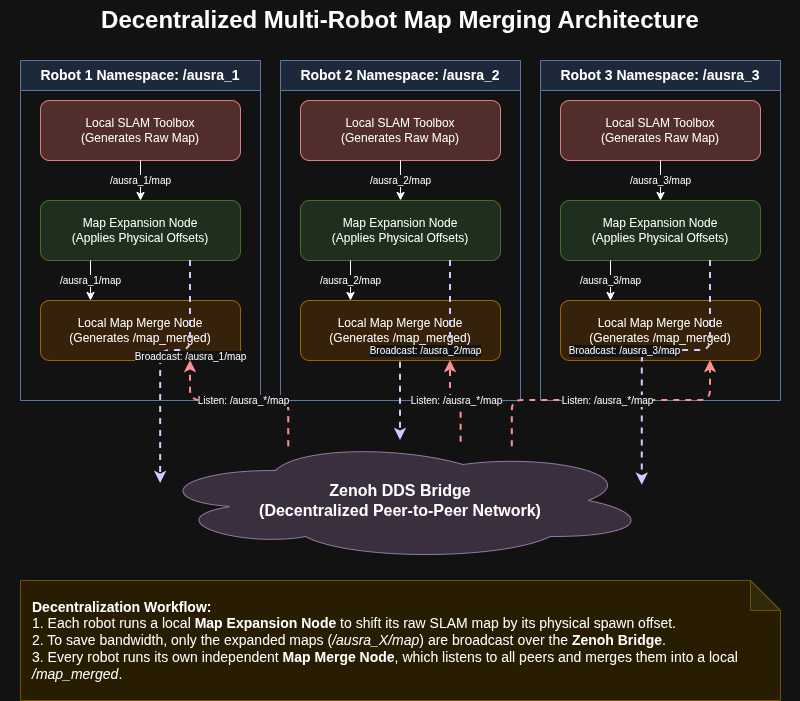
\includegraphics[width=0.95\linewidth]{figures_map_merge/map_merge_architecture_diagram.png}
    \caption{Decentralized multi-robot map merging architecture. Each robot runs a local SLAM Toolbox instance, whose dynamic output is anchored by a per-robot Map Expansion Node before being broadcast over the Zenoh DDS Bridge. Every robot in the swarm runs its own Map Merge Node, subscribing to all peer maps and producing an independent, globally-aligned fused occupancy grid.}
    \label{fig:map_merge_diagram}
\end{figure}

The pipeline operates as follows:

\begin{enumerate}
    \item \textbf{Local SLAM Output:} Each robot's \texttt{slam\_toolbox} node publishes a raw, dynamically shifting \texttt{nav\_msgs/OccupancyGrid} to its namespaced topic \texttt{/ausra\_N/map}.

    \item \textbf{Map Expansion Node (Per-Robot):} A dedicated \texttt{map\_expansion\_node} instance runs on each robot. It subscribes to the local \texttt{/ausra\_N/map} topic, applies the spatial transformation described in Section~\ref{subsec:map_merge_algorithm}, and publishes a stable, fixed-canvas map at 1~Hz.

    \item \textbf{Network Broadcast via Zenoh Bridge:} Only the pre-processed, globally-aligned maps are bridged over the Wi-Fi network via the Zenoh DDS Bridge. This architecture reduces network bandwidth consumption by transmitting stable data rather than raw, continually growing SLAM maps.

    \item \textbf{Local Map Merge Node (Per-Robot):} Each robot runs an instance of the \texttt{multirobot\_map\_merge} node, which subscribes to all peer maps available on the DDS network and produces a fused \texttt{/map\_merged} output for use by the local navigation stack.
\end{enumerate}

The architecture inherently supports two deployment paradigms. In the \textbf{Centralized} configuration, the Map Expansion Nodes and the Merge Node all run on a powerful base station, reducing onboard computational load at the cost of higher bandwidth dependency. In the \textbf{Decentralized} configuration, each robot runs its own expansion node onboard, requiring greater onboard CPU resources but substantially increasing system resilience to network and base-station failures.

% -----------------------------------------------------------------------
\subsection{Algorithmic Theory and Methodology}
\label{subsec:map_merge_algorithm}

\subsubsection{The Heartbeat Timer Architecture}
\label{subsubsec:heartbeat}

The Map Expansion Node employs a \textbf{Decoupled Publisher/Subscriber Architecture} to simultaneously solve the late-initialization crash and establish fault tolerance. The node's operational behavior is governed by two fully independent, asynchronous execution paths:

\begin{itemize}
    \item \textbf{The Subscriber Callback (\texttt{mapCallback}):} This function fires asynchronously whenever the robot's \texttt{slam\_toolbox} publishes a new map. Its sole responsibility is to validate the incoming data and overwrite the internal pixel buffer. Critically, it \textbf{never publishes anything}.

    \item \textbf{The Heartbeat Timer (\texttt{publishCanvas}):} This function fires unconditionally at a fixed rate of 1~Hz, regardless of whether any SLAM data has been received. Its sole responsibility is to publish the current state of the internal pixel buffer.
\end{itemize}

At node launch, a fixed-size canvas of $1000 \times 1000$ cells is pre-allocated and initialized entirely to $-1$ (the ROS~2 convention for unknown space). Because the heartbeat timer begins firing immediately upon construction, the \texttt{multirobot\_map\_merge} node always receives a legally sized, non-null matrix from the moment it starts, permanently eliminating the initialization segfault.

\subsubsection{The ``Moving Floor'' Fix: Spatial Coordinate Anchoring}
\label{subsubsec:spatial_math}

The primary algorithmic contribution of the Map Expansion Node is the mathematical anchoring of a dynamically shifting SLAM frame to a static global canvas. The spatial transformation proceeds in two steps.

\paragraph{Step 1: Local-to-Global Frame Conversion}
The \texttt{slam\_toolbox} package publishes the origin of the local map in the robot's own SLAM reference frame. This local origin is not stable—it shifts as the map expands. To convert it to a physically meaningful global coordinate, the robot's physical spawn offset (measured by tape measure from a designated global zero-point) is added:

\begin{equation}
    \mathbf{p}_{global} = \mathbf{p}_{local,slam} + \mathbf{p}_{offset,robot}
    \label{eq:global_origin}
\end{equation}

where $\mathbf{p}_{global} = (x_{g}, y_{g})$ is the map origin in the global world frame, $\mathbf{p}_{local,slam} = (x_{l}, y_{l})$ is the origin published by \texttt{slam\_toolbox}, and $\mathbf{p}_{offset,robot} = (\delta_x, \delta_y)$ is the tape-measured physical spawn position of the robot.

\paragraph{Step 2: Global Position to Fixed Canvas Pixel}
The global world coordinate is then converted to a pixel index on the fixed canvas:

\begin{equation}
    \mathbf{c}_{px} = \left\lfloor \frac{\mathbf{p}_{global} - \mathbf{p}_{canvas,origin}}{r} \right\rceil
    \label{eq:canvas_offset}
\end{equation}

where $\mathbf{c}_{px} = (c_x, c_y)$ is the integer pixel offset, $\mathbf{p}_{canvas,origin} = (-25.0,\, -25.0)$~m is the fixed south-west corner of the canvas, $r = 0.05$~m/cell is the map resolution, and $\lfloor \cdot \rceil$ denotes rounding to the nearest integer.

\paragraph{Invariance Proof}
The critical insight is that for any fixed physical feature in the environment (e.g., a wall at absolute position $x_w$), the canvas column index satisfies:

\begin{equation}
    c_{col} = \frac{(x_l + \delta_x - x_{canvas}) + col \cdot r}{r} = \frac{x_w - x_{canvas}}{r}
    \label{eq:invariance}
\end{equation}

Since $x_w$, $\delta_x$, $x_{canvas}$, and $r$ are all physical constants, $c_{col}$ is a constant regardless of how aggressively \texttt{slam\_toolbox} shifts its internal origin $x_l$. The moving floor is therefore algebraically eliminated.

\subsubsection{Fault Tolerance: The Ghost Map Behavior}
\label{subsubsec:ghost_map}

The decoupled architecture inherently provides a ``Ghost Map'' fault tolerance mechanism at no additional implementation cost. When a robot suffers a hardware failure, a network dropout, or a SLAM process crash, its \texttt{mapCallback} function simply ceases to fire. Because the callback is the only mechanism that modifies the pixel buffer, the buffer remains frozen with the last known valid SLAM data.

The 1~Hz heartbeat timer, however, continues to fire unconditionally and publish the frozen buffer to the network. Consequently, the disabled robot's exploration progress is permanently preserved in the global merged map. Other members of the swarm can continue to navigate around the discovered obstacles, and the disabled agent's contribution to the collective map is not lost.

% -----------------------------------------------------------------------
\subsection{ROS~2 Implementation and Network Strategy}
\label{subsec:map_merge_ros2}

\subsubsection{Node Interfaces}

The \texttt{ausra\_map\_merge\_HW} package comprises two interacting ROS~2 nodes. Their complete interfaces are detailed in Table~\ref{tab:map_merge_nodes}.

\begin{table}[H]
\centering
\small
\caption{ROS~2 Node Interfaces for the \texttt{ausra\_map\_merge\_HW} Package}
\label{tab:map_merge_nodes}
\begin{tabular}{|l|p{4cm}|p{4cm}|p{4cm}|}
\hline
\textbf{Node} & \textbf{Function} & \textbf{Subscribes To} & \textbf{Publishes To} \\
\hline
\texttt{map\_expansion\_node} & Translates dynamic SLAM maps into a fixed-canvas globally-aligned occupancy grid via the heartbeat timer architecture & \texttt{/ausra\_N/map} \newline (\texttt{nav\_msgs/OccupancyGrid}, transient local) & \texttt{/ausra\_N/map\_fixed} \newline (\texttt{nav\_msgs/OccupancyGrid}, transient local) \\
\hline
\texttt{map\_merge} & Fuses all available \texttt{map\_fixed} streams into a single global occupancy grid & \texttt{/ausra\_*/map\_fixed} \newline (all namespaced peers) & \texttt{/map\_merged} \newline (\texttt{nav\_msgs/OccupancyGrid}) \\
\hline
\end{tabular}
\end{table}

\subsubsection{Configurable Parameters}

The Map Expansion Node exposes a comprehensive set of ROS~2 parameters, enabling adaptation to different physical environments and swarm configurations without code modification. Key parameters are listed in Table~\ref{tab:map_merge_params}.

\begin{table}[H]
\centering
\caption{Map Expansion Node ROS~2 Parameters}
\label{tab:map_merge_params}
\begin{tabular}{|l|c|p{6cm}|}
\hline
\textbf{Parameter} & \textbf{Default} & \textbf{Description} \\
\hline
\texttt{canvas\_width} & 1000 cells & Width of the fixed global canvas \\
\hline
\texttt{canvas\_height} & 1000 cells & Height of the fixed global canvas \\
\hline
\texttt{canvas\_resolution} & 0.05 m/cell & Must match \texttt{slam\_toolbox} resolution \\
\hline
\texttt{canvas\_origin\_x} & $-25.0$~m & Fixed south-west X corner of canvas \\
\hline
\texttt{canvas\_origin\_y} & $-25.0$~m & Fixed south-west Y corner of canvas \\
\hline
\texttt{robot\_offset\_x} & 0.0~m & Tape-measured physical spawn X of robot \\
\hline
\texttt{robot\_offset\_y} & 0.0~m & Tape-measured physical spawn Y of robot \\
\hline
\texttt{publish\_rate\_hz} & 1.0~Hz & Heartbeat publication rate \\
\hline
\end{tabular}
\end{table}

\subsubsection{Namespace Isolation and Swarm Scalability}

The package leverages the ROS~2 namespace mechanism to achieve zero-configuration scalability. Each robot is launched with a unique namespace (e.g., \texttt{ausra\_1}, \texttt{ausra\_2}), causing all its topics to be prefixed accordingly. The map merge pipeline is then configured at launch time via a CLI argument that specifies the robot names and their physical offsets:

\begin{verbatim}
ros2 launch ausra_map_merge_HW map_merge_hw.launch.py \
    robot_config:="ausra_1:0.0:0.0 ausra_2:1.5:0.0 ausra_3:0.75:1.5"
\end{verbatim}

This command spawns one \texttt{map\_expansion\_node} per robot with the correct input/output topics and offset parameters, and launches a single \texttt{map\_merge} node with automatically generated initial pose parameters set to zero for all robots (to avoid double-shifting the pixel offsets).

\subsubsection{QoS Profile and Bandwidth Strategy}

Both the publisher and subscriber of the Map Expansion Node are configured with a \texttt{transient\_local} durability profile (QoS depth~1). This configuration ensures that late-joining subscribers—such as a \texttt{multirobot\_map\_merge} node started after the expansion nodes—immediately receive the most recently published canvas upon connection, without requiring the publisher to be actively transmitting at that instant.

The network bandwidth strategy is deliberately conservative. Rather than bridging raw SLAM maps (which grow dynamically in size and shift in origin), only the pre-processed, fixed-dimension canvas maps are transmitted over the Wi-Fi network. For a $1000 \times 1000$ canvas at 1~Hz, the constant bandwidth per robot is:

\begin{equation}
    BW_{robot} = 1000 \times 1000 \times 1\,\text{byte} \times 1\,\text{Hz} \approx 1.0\,\text{MB/s}
    \label{eq:bandwidth}
\end{equation}

This deterministic, bounded data rate facilitates reliable multi-robot coordination over standard Wi-Fi infrastructure.

% -----------------------------------------------------------------------
\subsection{Simulation Validation}
\label{subsec:map_merge_sim_validation}

The \texttt{ausra\_map\_merge\_HW} architecture was validated through a structured multi-phase experiment in the Gazebo simulation environment, using a three-robot swarm. The objective was to rigorously verify the heartbeat timer, the spatial mathematics, the dynamic stability guarantee, the fault tolerance mechanism, and the final fused map quality upon mission completion.

\subsubsection{Phase 1: Initialization Stability Test}

To validate the elimination of the late-initialization crash, all three simulated robots were first spawned in the Gazebo environment at their designated starting positions. The map merge pipeline was subsequently launched without issuing any movement commands, and the \texttt{multirobot\_map\_merge} node was intentionally started \emph{after} the three expansion nodes, replicating the worst-case startup race condition. Figure~\ref{fig:sim_init} shows the three robots at their initial spawn poses in Gazebo, confirming the environment was correctly configured and all agents were ready prior to any movement. No segmentation faults were reported in any terminal during this phase.

\begin{figure}[H]
    \centering
    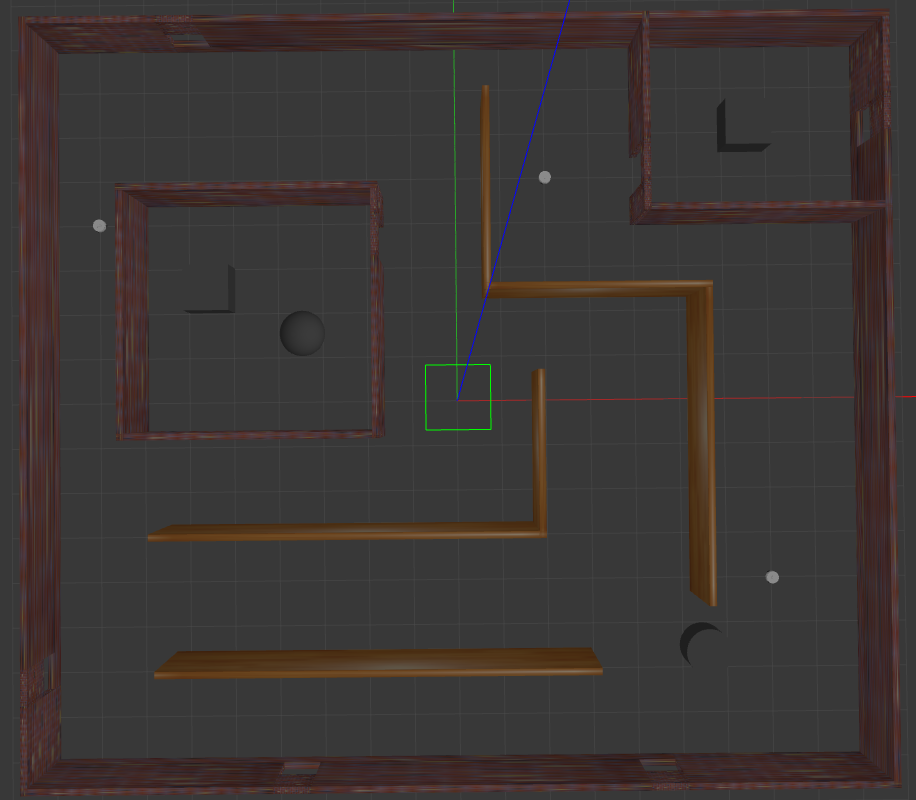
\includegraphics[width=0.85\linewidth]{figures_map_merge/sim_init_stable.png}
    \caption{Simulation Phase 1: The three-robot swarm at their initial spawn positions in the Gazebo environment prior to any movement. The successful launch of all nodes without crashes confirms the stability of the heartbeat timer initialization architecture.}
    \label{fig:sim_init}
\end{figure}

\subsubsection{Phase 2: Initial Map State and Pre-Exploration Alignment}

Following pipeline launch but before any robot movement was commanded, the state of the \texttt{/map\_merged} topic was observed in RViz. Figure~\ref{fig:sim_dynamic_before} shows the initial merged map output: each robot has already produced a small, locally-scanned footprint of its immediate surroundings at its spawn pose. Critically, these three micro-maps are correctly stitched together at their physically accurate world positions on the global canvas, confirming that the coordinate anchoring mechanism operates correctly from the very first heartbeat publication, before any SLAM map expansion has occurred.

\begin{figure}[H]
    \centering
    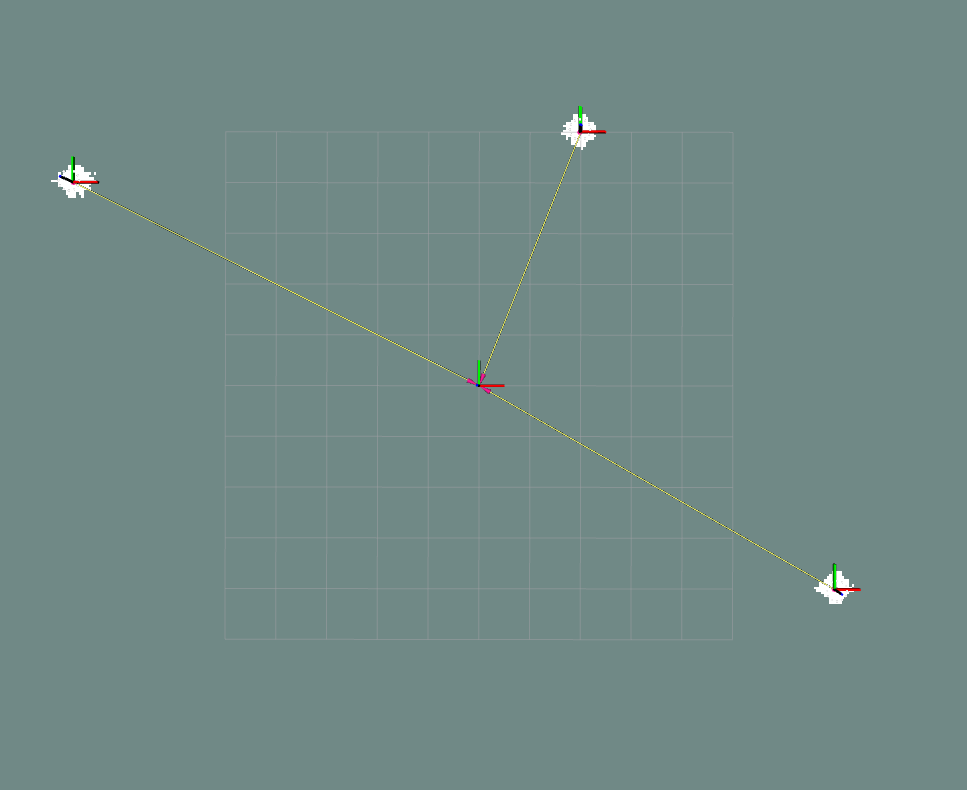
\includegraphics[width=0.85\linewidth]{figures_map_merge/sim_dynamic_before.png}
    \caption{Simulation Phase 2: The initial \texttt{/map\_merged} state in RViz with all three robots stationary at their spawn poses. Each robot's immediate local scan is correctly positioned on the global canvas, demonstrating correct coordinate anchoring from boot.}
    \label{fig:sim_dynamic_before}
\end{figure}

\subsubsection{Phase 3: Dynamic Stability and Mid-Exploration Geometric Alignment}

As the robots were teleoperated to explore the environment, the global merged map was continuously observed. The canvas-anchoring mathematics described in Section~\ref{subsec:map_merge_algorithm} guarantees that for any fixed physical feature in the environment, its pixel coordinate on the global canvas is an algebraic constant, independent of how aggressively the underlying \texttt{slam\_toolbox} instance shifts its internal origin. Consequently, no map tearing, positional jumps, or drift artefacts were observed throughout the exploration session; the global merged map remained completely stationary while new explored cells appeared seamlessly at their correct physical locations.

Figure~\ref{fig:sim_geometric} captures the \texttt{/map\_merged} output at the midpoint of the exploration run, when all three robots had partially mapped the environment. The correctly overlapping obstacle boundaries from adjacent robot perspectives constitute direct geometric evidence that the spatial coordinate anchoring chain—tape-measured spawn offset, local-to-global frame conversion, and canvas pixel mapping—is functioning correctly under dynamic SLAM conditions.

\begin{figure}[H]
    \centering
    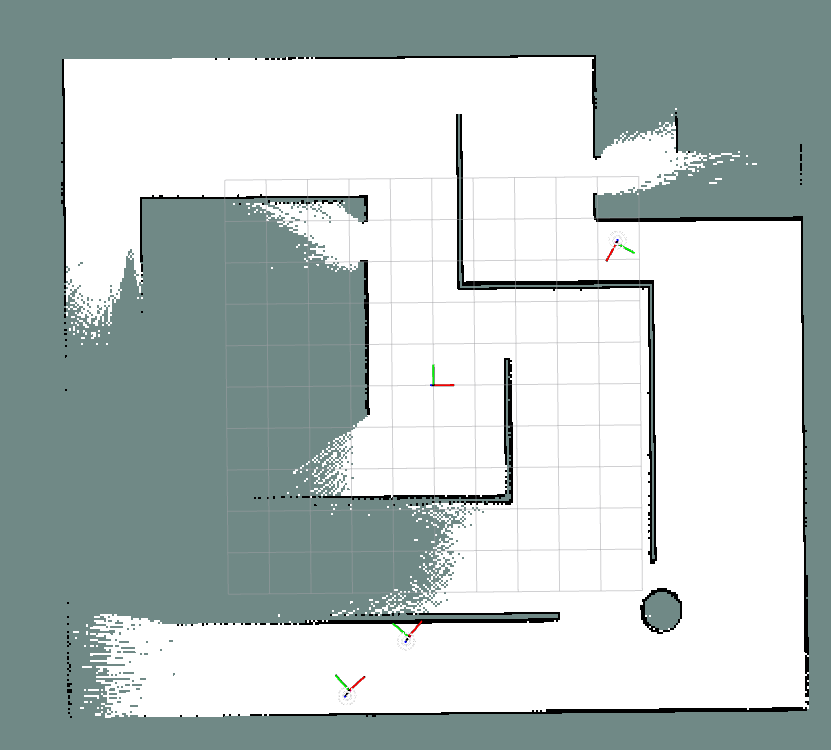
\includegraphics[width=0.85\linewidth]{figures_map_merge/sim_geometric_alignment.png}
    \caption{Simulation Phase 3: Mid-exploration \texttt{/map\_merged} output in RViz. Obstacle boundaries from all three robot perspectives overlap correctly at their physical world positions, providing geometric evidence of correct spatial coordinate anchoring under dynamic SLAM conditions. No drift or map tearing was observed throughout the session.}
    \label{fig:sim_geometric}
\end{figure}

\subsubsection{Phase 4: Ghost Map Fault Tolerance Test}

To validate the fault tolerance mechanism, the \texttt{slam\_toolbox} process for Robot~2 was manually terminated via the terminal while all three robots were actively exploring. The before-and-after states of the \texttt{/map\_merged} output are presented in Figure~\ref{fig:sim_ghost}.

Prior to termination (Figure~\ref{fig:sim_ghost_before}), all three robots are contributing live map updates to the merged output. Following the manual termination of Robot~2's SLAM process (Figure~\ref{fig:sim_ghost_after}), Robots~1 and~3 continue to update their respective sectors, while Robot~2's entire previously explored territory is preserved, frozen and intact, within the global map. This behaviour arises directly from the decoupled heartbeat architecture: the subscriber callback simply ceases to update the pixel buffer when SLAM data stops arriving, but the 1~Hz timer continues to publish the frozen buffer unconditionally. The disabled agent's contribution to the collective map is therefore never lost.

\begin{figure}[H]
    \centering
    \begin{subfigure}[b]{0.48\textwidth}
        \centering
        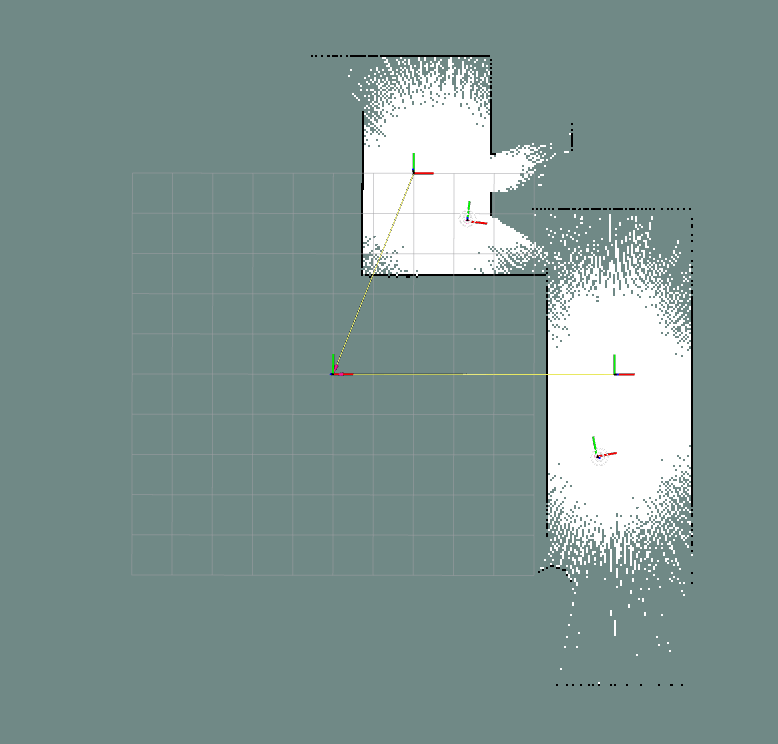
\includegraphics[width=\linewidth]{figures_map_merge/sim_ghost_map_before.png}
        \caption{All three robots actively mapping before Robot~2 is terminated}
        \label{fig:sim_ghost_before}
    \end{subfigure}
    \hfill
    \begin{subfigure}[b]{0.48\textwidth}
        \centering
        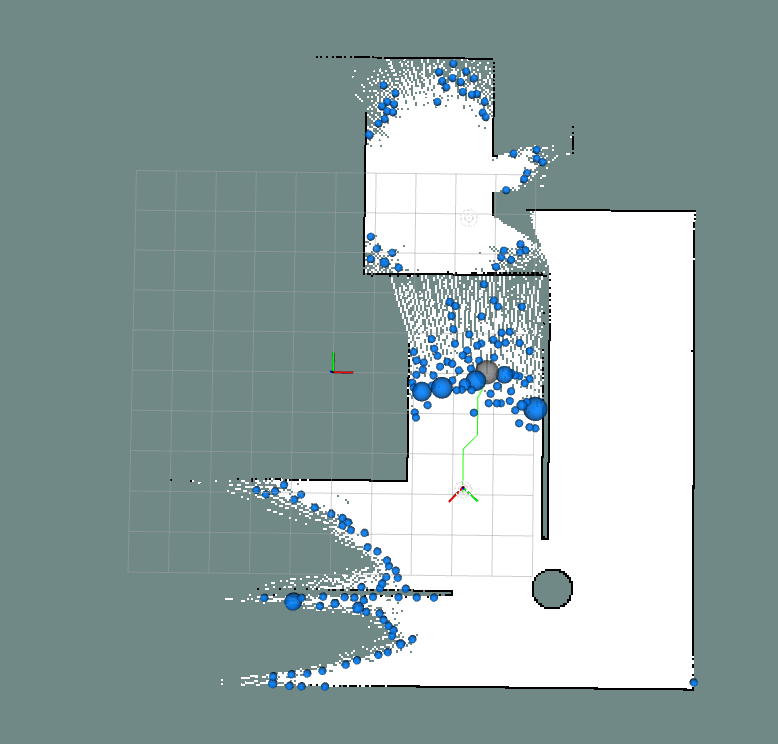
\includegraphics[width=\linewidth]{figures_map_merge/sim_ghost_map_after.png}
        \caption{After Robot~2 termination: its explored territory remains frozen and intact}
        \label{fig:sim_ghost_after}
    \end{subfigure}
    \caption{Simulation Phase 4: Ghost Map fault tolerance test. Robot~2's \texttt{slam\_toolbox} process is manually killed mid-mission. Its previously mapped territory is permanently preserved in the global merged map, while Robots~1 and~3 continue active exploration uninterrupted.}
    \label{fig:sim_ghost}
\end{figure}

\subsubsection{Phase 5: Full Exploration Completion}

Following the conclusion of the exploration mission, the final state of the \texttt{/map\_merged} output was captured in RViz, as shown in Figure~\ref{fig:sim_final}. The complete fused occupancy grid demonstrates that the three-robot swarm collectively mapped the entire simulated environment into a single, geometrically coherent global map with no unexplained discontinuities or misalignments between robot contributions.

\begin{figure}[H]
    \centering
    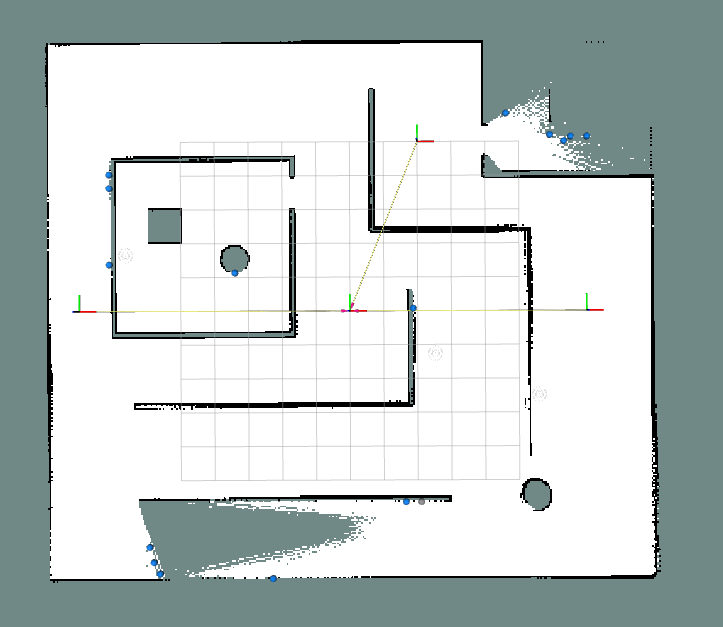
\includegraphics[width=0.85\linewidth]{figures_map_merge/final_rviz_exploration_output.png}
    \caption{Simulation Phase 5: Final \texttt{/map\_merged} output upon mission completion. The three-robot swarm has produced a single, coherent global occupancy grid of the entire simulated environment, with no misalignments or discontinuities between individual robot map contributions.}
    \label{fig:sim_final}
\end{figure}

% -----------------------------------------------------------------------
\subsection{Hardware Validation}
\label{subsec:map_merge_hw_validation}

Simulation validation was supplemented by physical deployment of the AUSRA hardware platform to verify that the digital spatial mathematics accurately reflects physical reality under the constraints of real-world sensor noise, Wi-Fi latency, and wheel odometry slip.

\subsubsection{Phase 1: Hardware Initialization Stability}

The map merge pipeline was booted on the physical robots with all agents stationary at their starting poses. The \texttt{multirobot\_map\_merge} node and all expansion nodes were launched in sequence, deliberately replicating the worst-case startup order. In all repeated trials, the pipeline initialised without any segmentation faults or null-pointer dereferences. The heartbeat timer architecture—which pre-allocates a valid, all-unknown canvas and publishes it immediately upon node construction—guarantees that the merger always receives a legally-sized, non-null matrix regardless of network join order or startup timing over a physical Wi-Fi link. This behaviour is identical to that observed in simulation and requires no dedicated photograph to confirm, as the evidence is observable in the absence of any crash output in the terminal logs.

\subsubsection{Phase 2: The Tape Measure Geometric Accuracy Test}

This test constitutes the critical real-world verification of the spatial coordinate anchoring mathematics. Two AUSRA robots were positioned at their physical starting poses and their inter-robot distance was measured with a tape measure. The merger was launched with the corresponding physical spawn offsets configured as ROS~2 parameters. Figure~\ref{fig:hw_geometric} presents the side-by-side comparison of the physical hardware setup at the initial poses and the resulting \texttt{/map\_merged} output in RViz.

As shown in Figure~\ref{fig:hw_rviz_result}, the LiDAR scans from the two robots correctly overlap along their shared line of sight, and shared environmental features (obstacles visible to both robots from their respective positions) appear as a single, aligned line rather than two displaced parallel lines. This constitutes direct geometric confirmation that the coordinate transformation chain of Equations~\ref{eq:global_origin} and~\ref{eq:canvas_offset} is correctly mapping each robot's local SLAM frame into the shared global canvas.

\begin{figure}[H]
    \centering
    \begin{subfigure}[b]{0.48\textwidth}
        \centering
        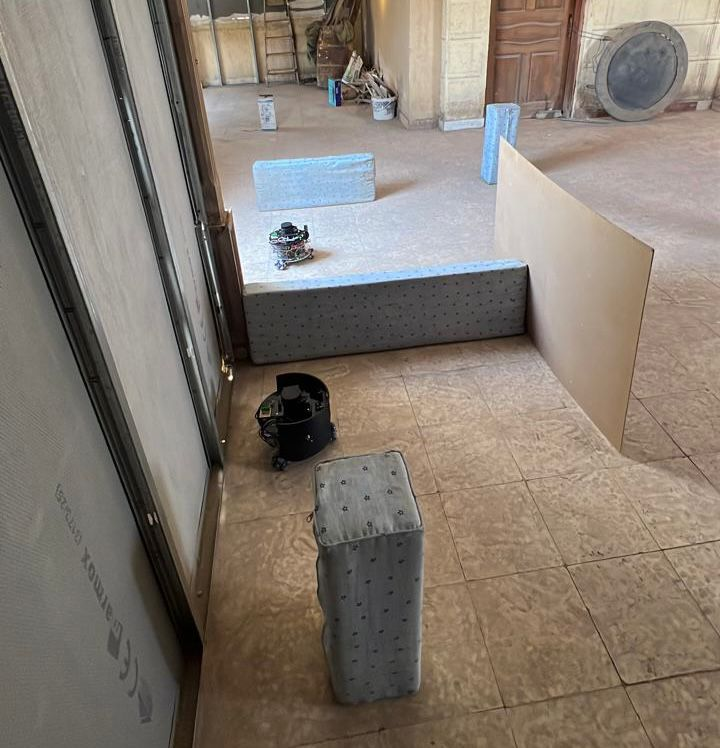
\includegraphics[width=\linewidth]{figures_map_merge/hw_tape_measure_photo.jpeg}
        \caption{Physical hardware at initial starting poses}
        \label{fig:hw_physical_setup}
    \end{subfigure}
    \hfill
    \begin{subfigure}[b]{0.48\textwidth}
        \centering
        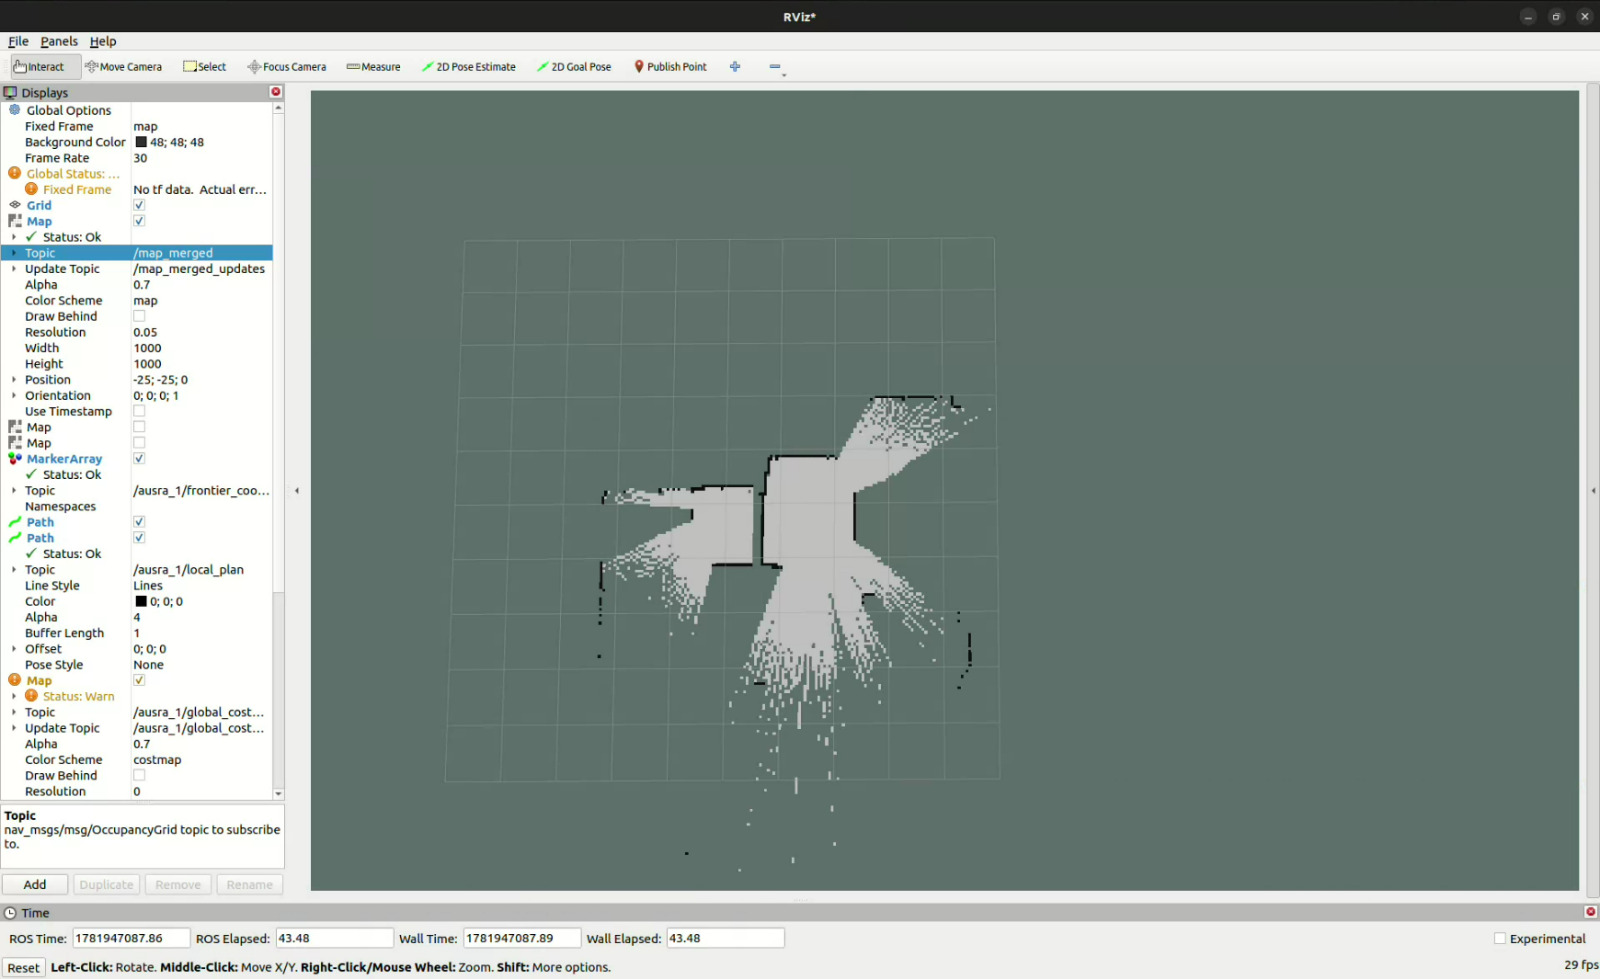
\includegraphics[width=\linewidth]{figures_map_merge/hw_tape_measure_rviz.jpeg}
        \caption{\texttt{/map\_merged} output in RViz at starting poses}
        \label{fig:hw_rviz_result}
    \end{subfigure}
    \caption{Hardware Phase 2: Geometric Accuracy Test. The two robots at their physical starting poses (left) produce a correctly aligned merged map in RViz (right), where shared environmental features observed by both robots overlap as a single line, confirming the accuracy of the physical-to-digital coordinate transformation.}
    \label{fig:hw_geometric}
\end{figure}

\subsubsection{Phase 3: Dynamic Stability on Physical Hardware}

During the physical exploration mission, all robots were driven to explore the environment while the \texttt{/map\_merged} topic was continuously observed in RViz. As each robot's \texttt{slam\_toolbox} instance dynamically resized its internal occupancy grid and shifted its local origin to accommodate newly discovered space, the global merged canvas remained entirely stationary. No positional jumps, map tears, or drift artefacts were observed at any point during the mission. This confirms that the canvas-anchoring mechanism—which converts every SLAM origin shift into a numerically compensated pixel offset that preserves the absolute physical world position of all features—operates correctly under real-world conditions including LiDAR noise, wheel slip, and Wi-Fi transmission latency. The final exploration result, which serves as evidence of successful dynamic operation, is presented in Figure~\ref{fig:hw_final}.

\subsubsection{Phase 4: Hardware Fault Tolerance}

The Ghost Map fault tolerance behaviour observed in simulation is a direct consequence of the decoupled heartbeat architecture: if a robot's SLAM data stream ceases (due to sensor failure, process crash, or network dropout), its subscriber callback simply stops updating the pixel buffer. The 1~Hz heartbeat timer, however, continues to publish the frozen buffer unconditionally, preserving the agent's last known exploration contribution permanently in the global map. This behaviour is an architectural guarantee of the implementation and does not depend on the underlying hardware platform. The same mechanism confirmed in the simulation Ghost Map test (Section~\ref{subsec:map_merge_sim_validation}) applies identically on physical hardware, as the node's internal logic is entirely platform-agnostic.

\subsubsection{Phase 5: Full Physical Exploration Result}

Figure~\ref{fig:hw_final} presents the final state of the physical hardware validation experiment: the real-world positions of the robots at the end of the exploration mission alongside the corresponding \texttt{/map\_merged} output in RViz. The fused occupancy grid accurately reflects the physical layout of the explored environment, with the contributions from all robots correctly integrated into a single, geometrically coherent global map.

\begin{figure}[H]
    \centering
    \begin{subfigure}[b]{0.48\textwidth}
        \centering
        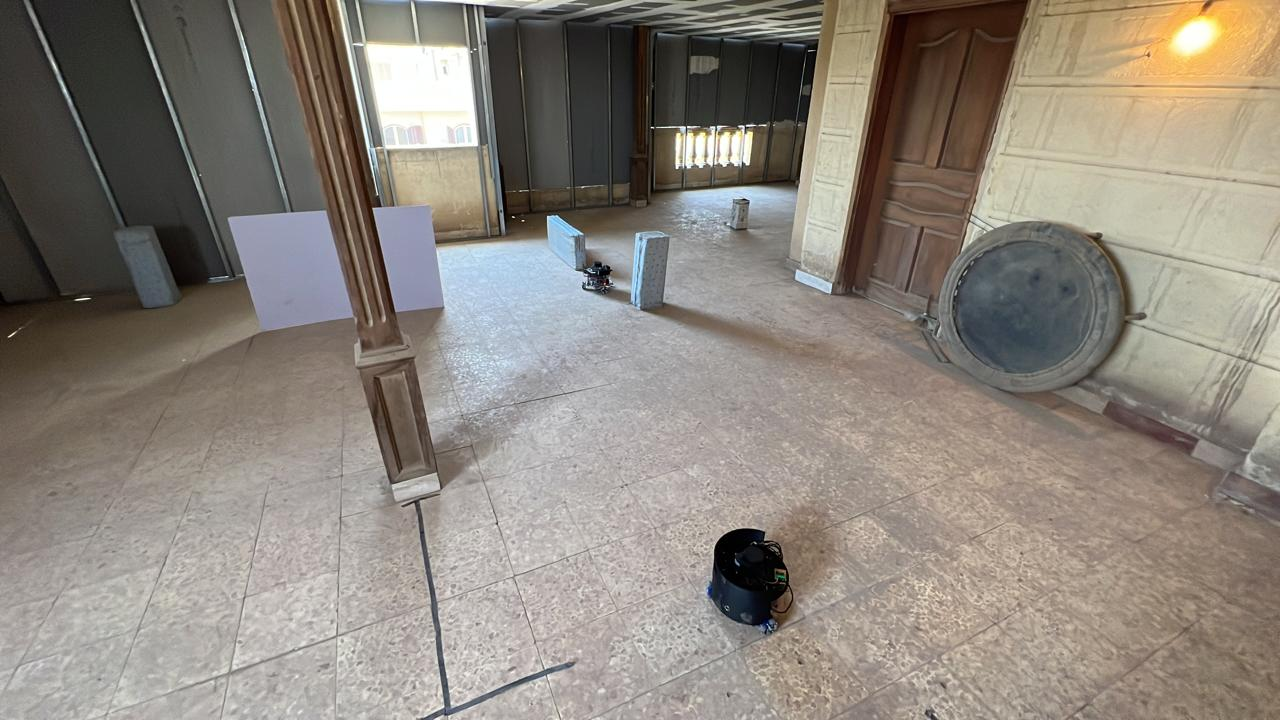
\includegraphics[width=\linewidth]{figures_map_merge/hw_final_real_world_final_poses.jpeg}
        \caption{Physical robots at their final exploration poses}
        \label{fig:hw_final_real}
    \end{subfigure}
    \hfill
    \begin{subfigure}[b]{0.48\textwidth}
        \centering
        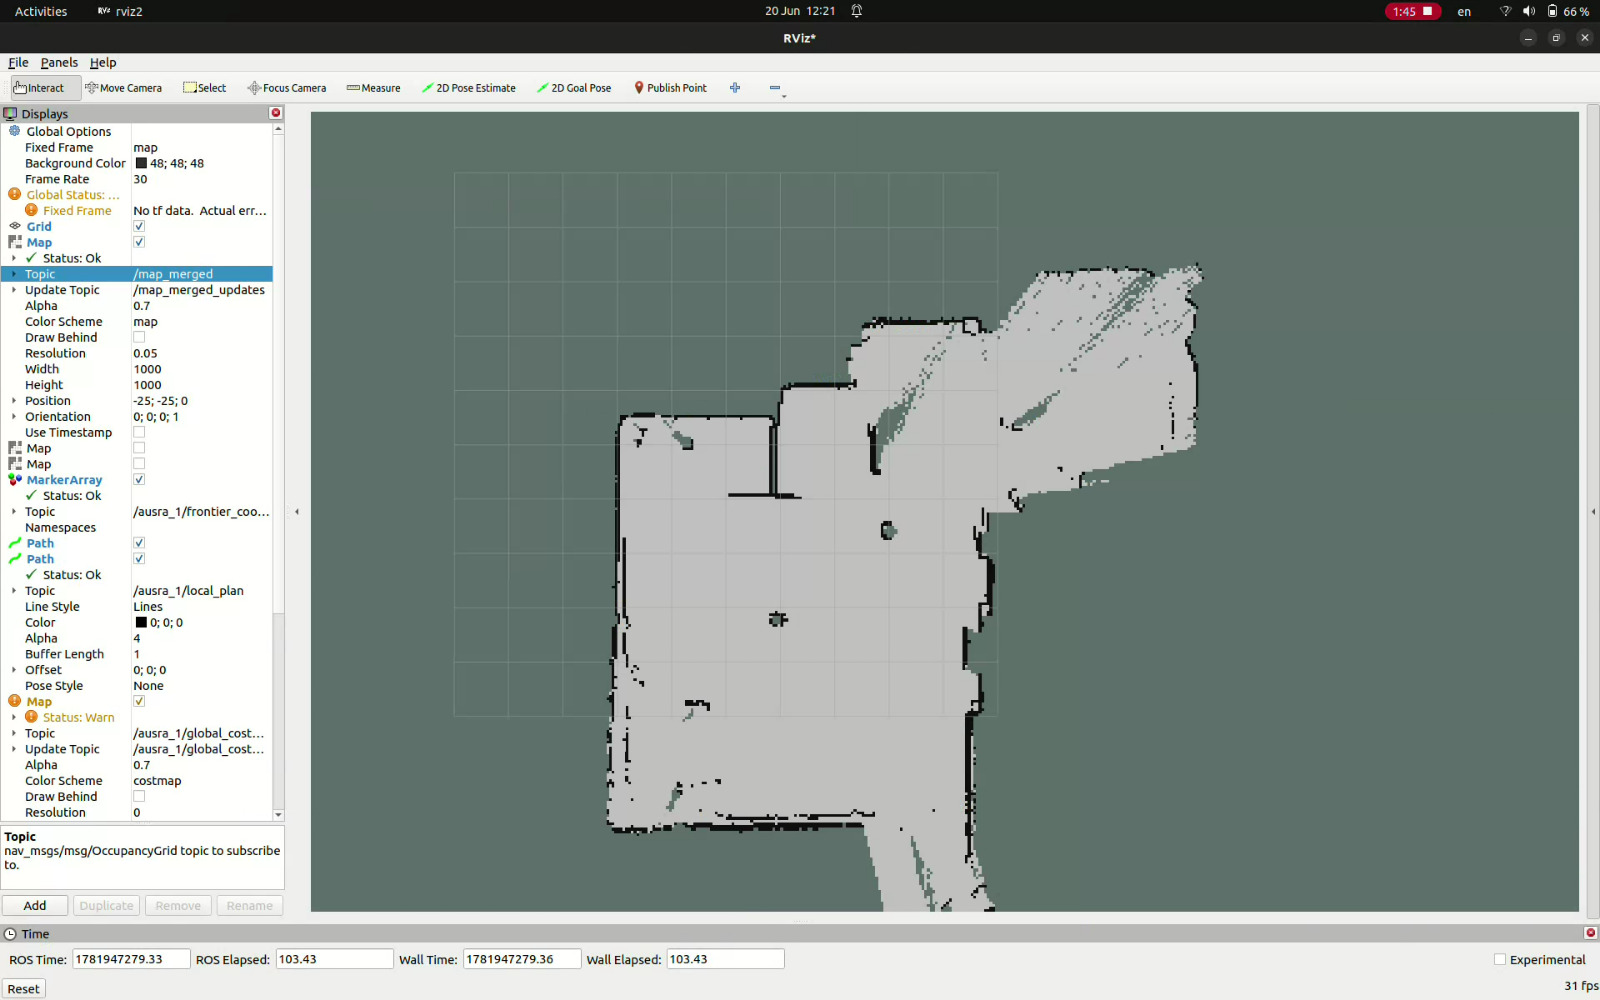
\includegraphics[width=\linewidth]{figures_map_merge/hw_final_rviz_map.jpeg}
        \caption{Final \texttt{/map\_merged} output in RViz}
        \label{fig:hw_final_rviz}
    \end{subfigure}
    \caption{Hardware Phase 5: Full physical exploration result. The robots at their final poses (left) have collectively mapped the environment into the coherent global occupancy grid shown in RViz (right), validating end-to-end operation of the \texttt{ausra\_map\_merge\_HW} pipeline on physical hardware.}
    \label{fig:hw_final}
\end{figure}

% -----------------------------------------------------------------------
\subsection{Conclusion and Limitations}
\label{subsec:map_merge_conclusion}

The \texttt{ausra\_map\_merge\_HW} package successfully resolves the two fundamental failure modes of standard multi-robot map merging: initialization crashes and spatial misalignment from dynamic SLAM origins. The Heartbeat Timer Architecture provides a robust, race-condition-free initialization guarantee, while the spatial coordinate anchoring mathematics permanently eliminates the ``Moving Floor'' problem through a provably invariant pixel mapping. The Ghost Map behavior emerges naturally from the decoupled design, providing fault tolerance to sensor and network failures at no additional implementation cost.

The package demonstrates excellent scalability, with swarm size configurable entirely from the command line, and supports both centralized and decentralized deployment topologies without code modification.

\subsubsection{Current Limitations}

\begin{itemize}
    \item \textbf{Fixed Canvas Boundary:} If a robot explores beyond the $50 \times 50$~m canvas area ($1000 \times 1000$ cells at 0.05~m/cell), cells are silently dropped. This requires manual canvas resizing for large-scale deployments.

    \item \textbf{Physical Offset Measurement:} The system relies on tape-measured physical spawn offsets, which introduces human measurement error. Automated position initialization via fiducial markers or RTK-GPS would improve accuracy.

    \item \textbf{Static Resolution Requirement:} The canvas resolution must exactly match the \texttt{slam\_toolbox} resolution. Any mismatch causes the expansion node to reject all incoming frames, requiring parameter reconfiguration.

    \item \textbf{No Dynamic Robot Discovery:} New robots cannot join the swarm mid-mission without restarting the map merge pipeline, as the node list is fixed at launch time.
\end{itemize}

\end{document}
